\subsection{Vehicle Detection Model Evaluation}

Two YOLOv8 models were developed for object detection under different lighting conditions: daytime and nighttime. This section presents the training results, accuracy metrics, and validation outcomes for each model.

\subsubsection{Daytime Model Training Results}

The YOLOv8 model was trained using images captured during daylight over 250 epochs. Key metrics such as precision, recall, and mAP50 were recorded at selected checkpoints, as shown in Table~\ref{table:akurasi_model_siang}.

\begin{table}[H]
\caption{Training Accuracy of Daytime Detection Model}
\label{table:akurasi_model_siang}
\centering
\begin{tabular}{|c|c|c|c|}
\hline
\textbf{Epochs} & \textbf{Precision} & \textbf{Recall} & \textbf{mAP50} \\ \hline
50 & 0.67893 & 0.68114 & 0.6863 \\ \hline
100 & 0.76356 & 0.77383 & 0.72166 \\ \hline
160 (best) & 0.80555 & 0.79315 & 0.82471 \\ \hline
200 & 0.79412 & 0.76758 & 0.77683 \\ \hline
250 & 0.79412 & 0.76758 & 0.77683 \\ \hline
\end{tabular}
\end{table}

Figure~\ref{fig:grafik_model_siang} illustrates the training curves for bounding box loss, classification loss, and average precision.

\begin{figure}[H]
\centering
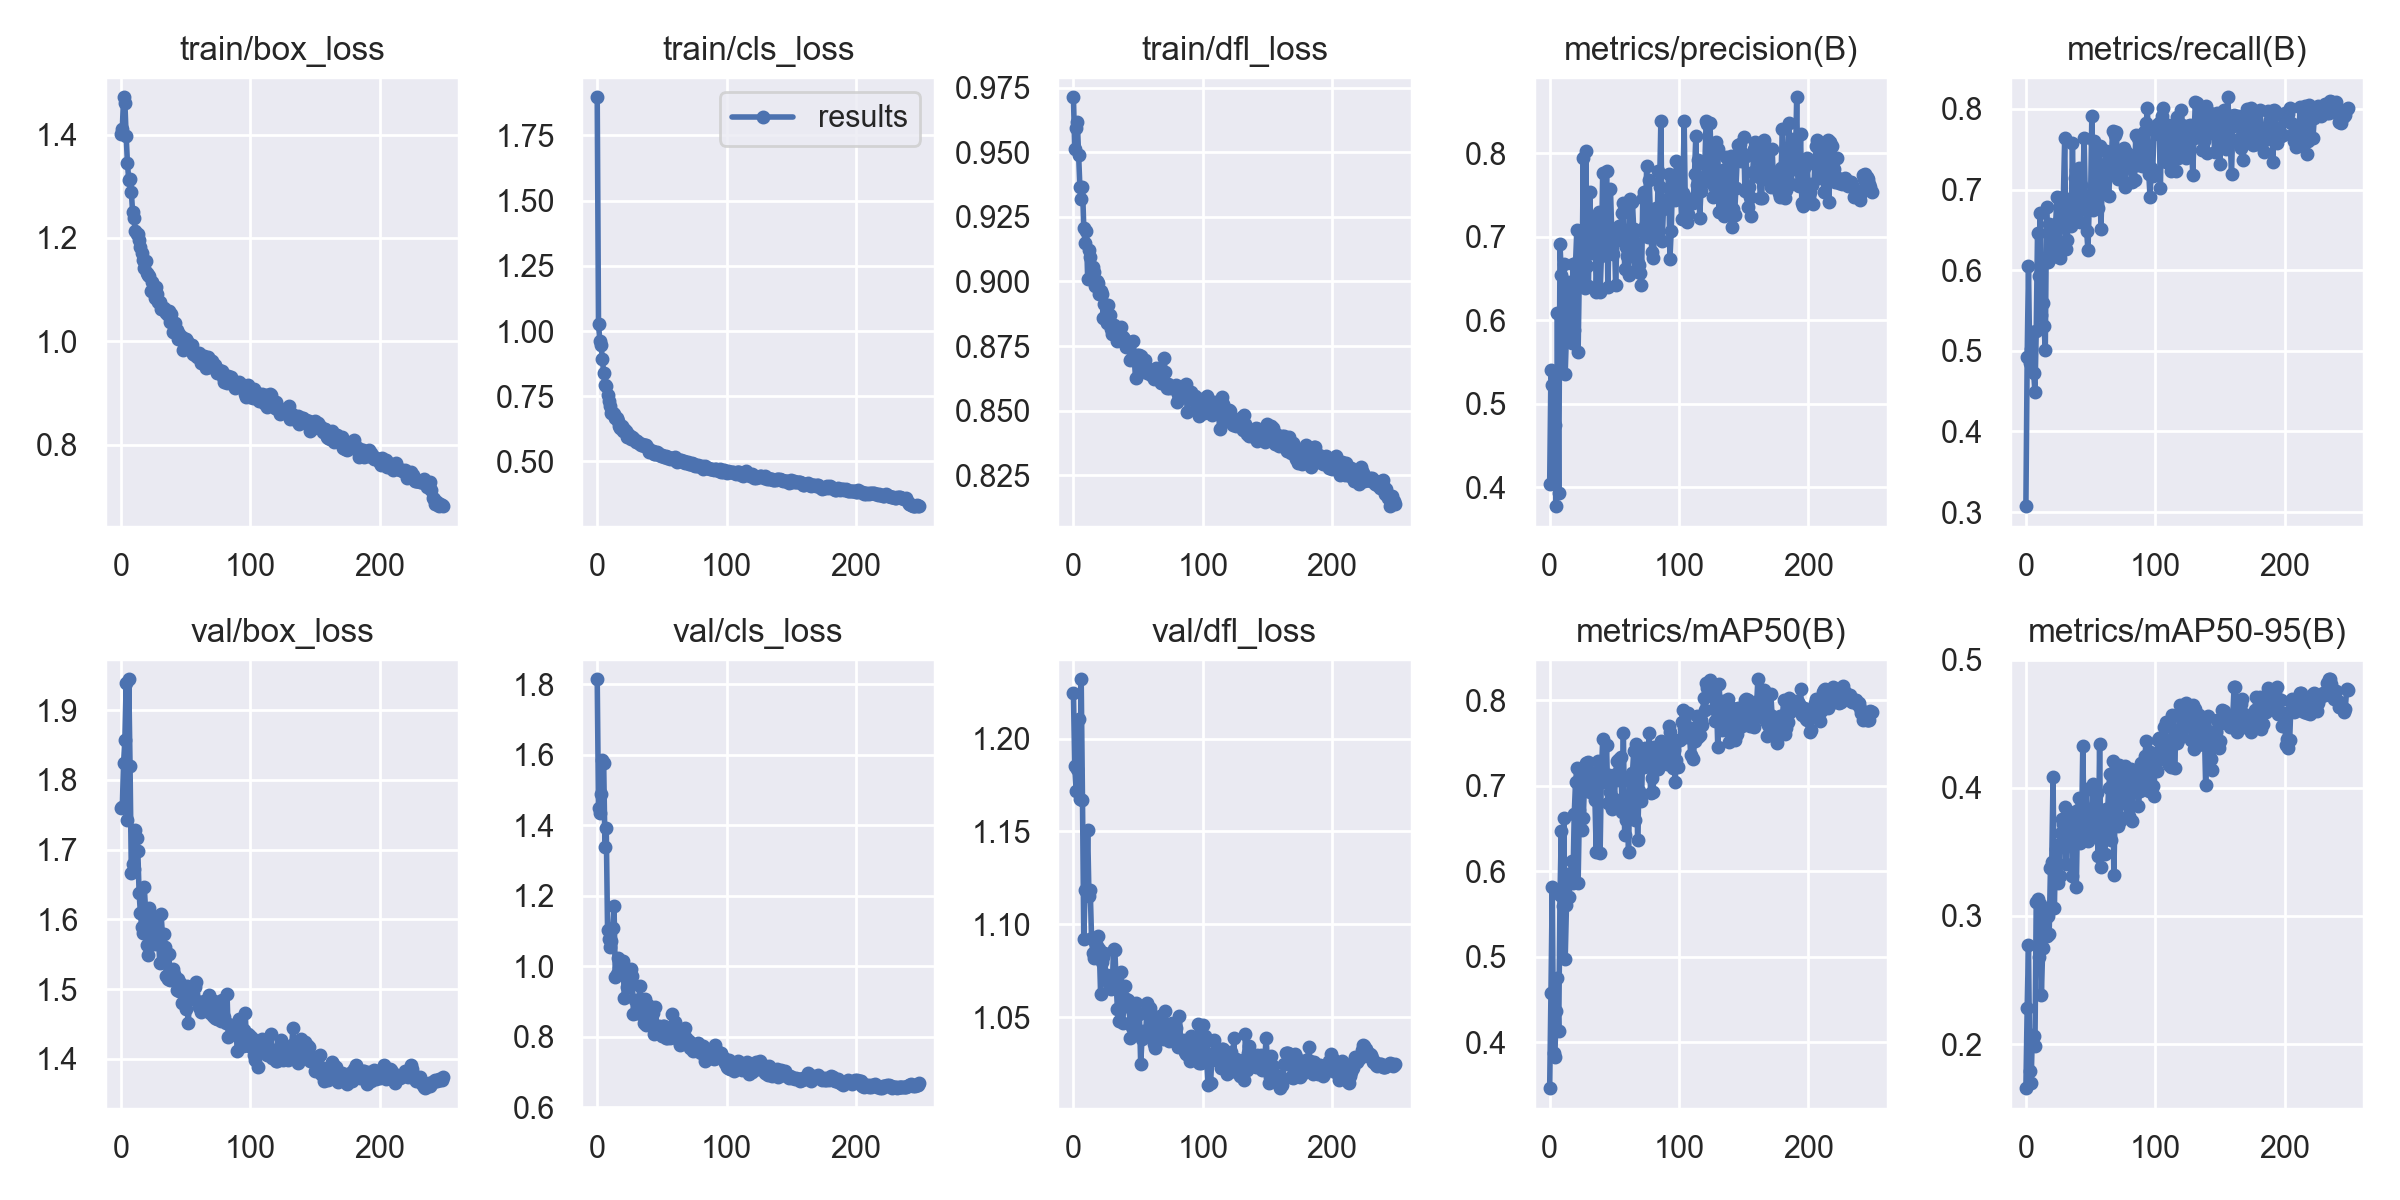
\includegraphics[width=0.45\textwidth]{gambar/results_siang.png}
\caption{Training curves for the daytime YOLOv8 model.}
\label{fig:grafik_model_siang}
\end{figure}

The confusion matrix in Figure~\ref{fig:confusion_matrix_siang} shows classification accuracy across object categories: car, motorcycle, truck, and background.

\begin{figure}[H]
\centering
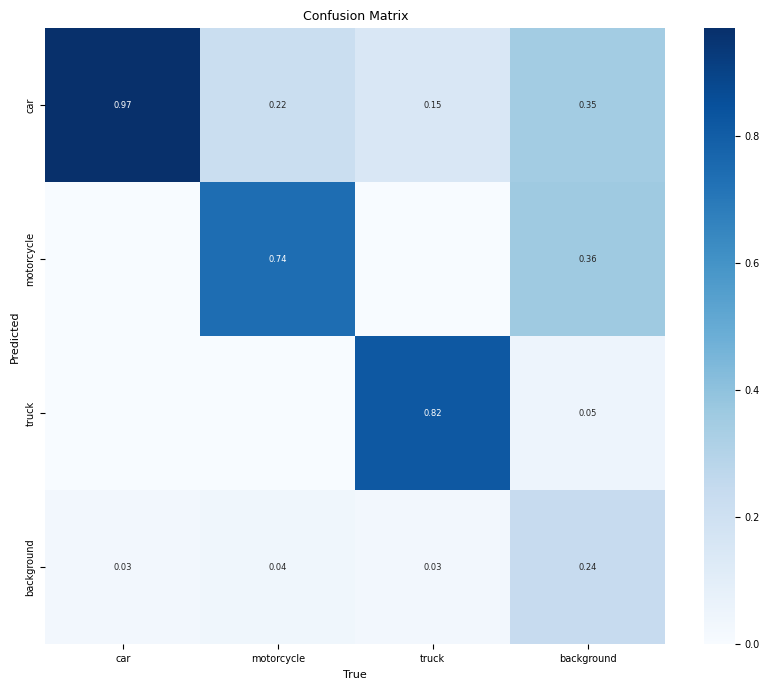
\includegraphics[width=0.45\textwidth]{gambar/confusion_siang.png}
\caption{Confusion matrix of the daytime detection model.}
\label{fig:confusion_matrix_siang}
\end{figure}

\begin{itemize}
    \item \textbf{Car:} 97\% correctly classified; minor confusion with background.
    \item \textbf{Motorcycle:} 74\% correct; 22\% misclassified as car.
    \item \textbf{Truck:} 82\% correct; minor confusion with background and car.
    \item \textbf{Background:} Model struggled, with frequent misclassification.
\end{itemize}

Validation results in Figure~\ref{fig:validasi_siang} show bounding boxes with confidence scores above 0.5.

\begin{figure}[H]
\centering
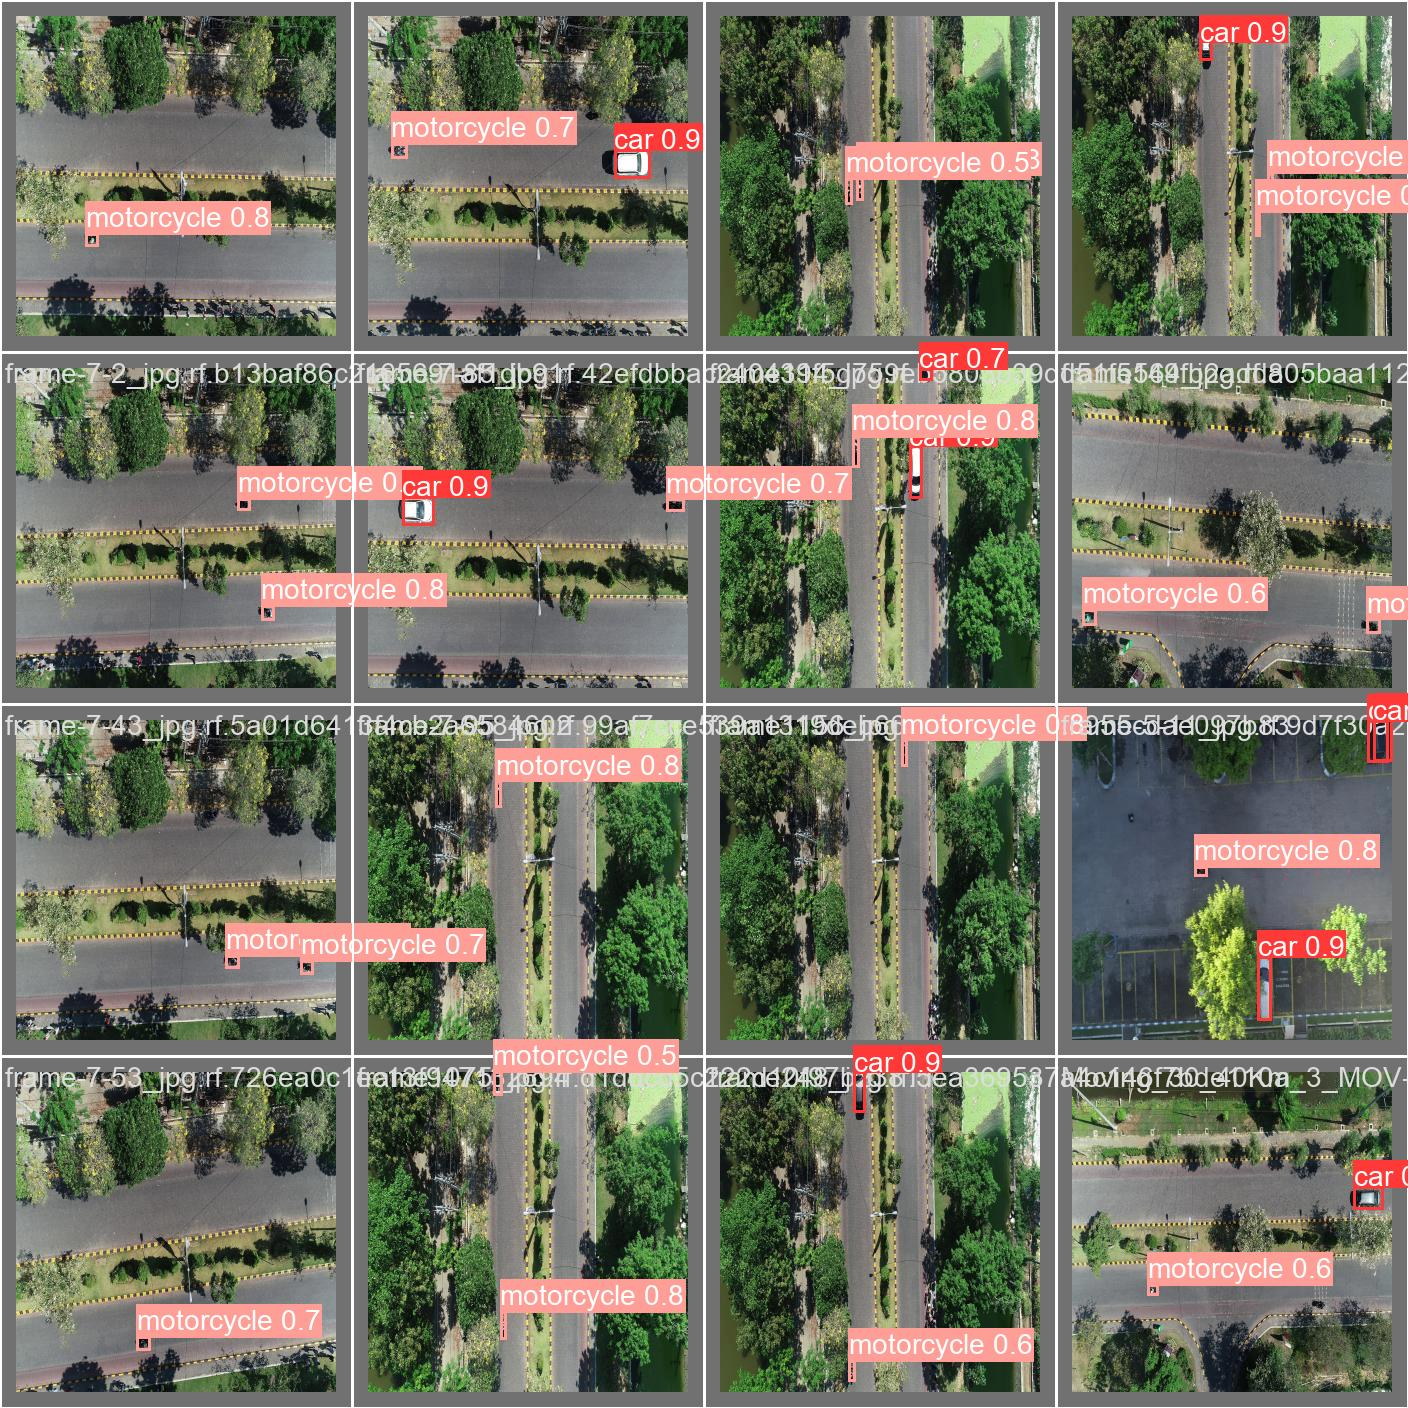
\includegraphics[width=0.45\textwidth]{gambar/val_batch_siang.jpg}
\caption{Validation results for the daytime model.}
\label{fig:validasi_siang}
\end{figure}

\subsubsection{Nighttime Model Training Results}

The nighttime model was trained on a low-light dataset for 250 epochs. Performance metrics are summarized in Table~\ref{table:akurasi_model_malam}.

\begin{table}[H]
\caption{Training Accuracy of Nighttime Detection Model}
\label{table:akurasi_model_malam}
\centering
\begin{tabular}{|c|c|c|c|}
\hline
\textbf{Epochs} & \textbf{Precision} & \textbf{Recall} & \textbf{mAP50} \\ \hline
50 & 0.81247 & 0.8977 & 0.81938 \\ \hline
72 (best) & 0.94688 & 0.88395 & 0.92997 \\ \hline
100 & 0.95264 & 0.88435 & 0.90664 \\ \hline
200 & 0.9409 & 0.89202 & 0.90600 \\ \hline
250 & 0.92616 & 0.88637 & 0.88913 \\ \hline
\end{tabular}
\end{table}

The training graphs in Figure~\ref{fig:grafik_model_malam} show steady improvements in both loss functions and detection metrics.

\begin{figure}[H]
\centering
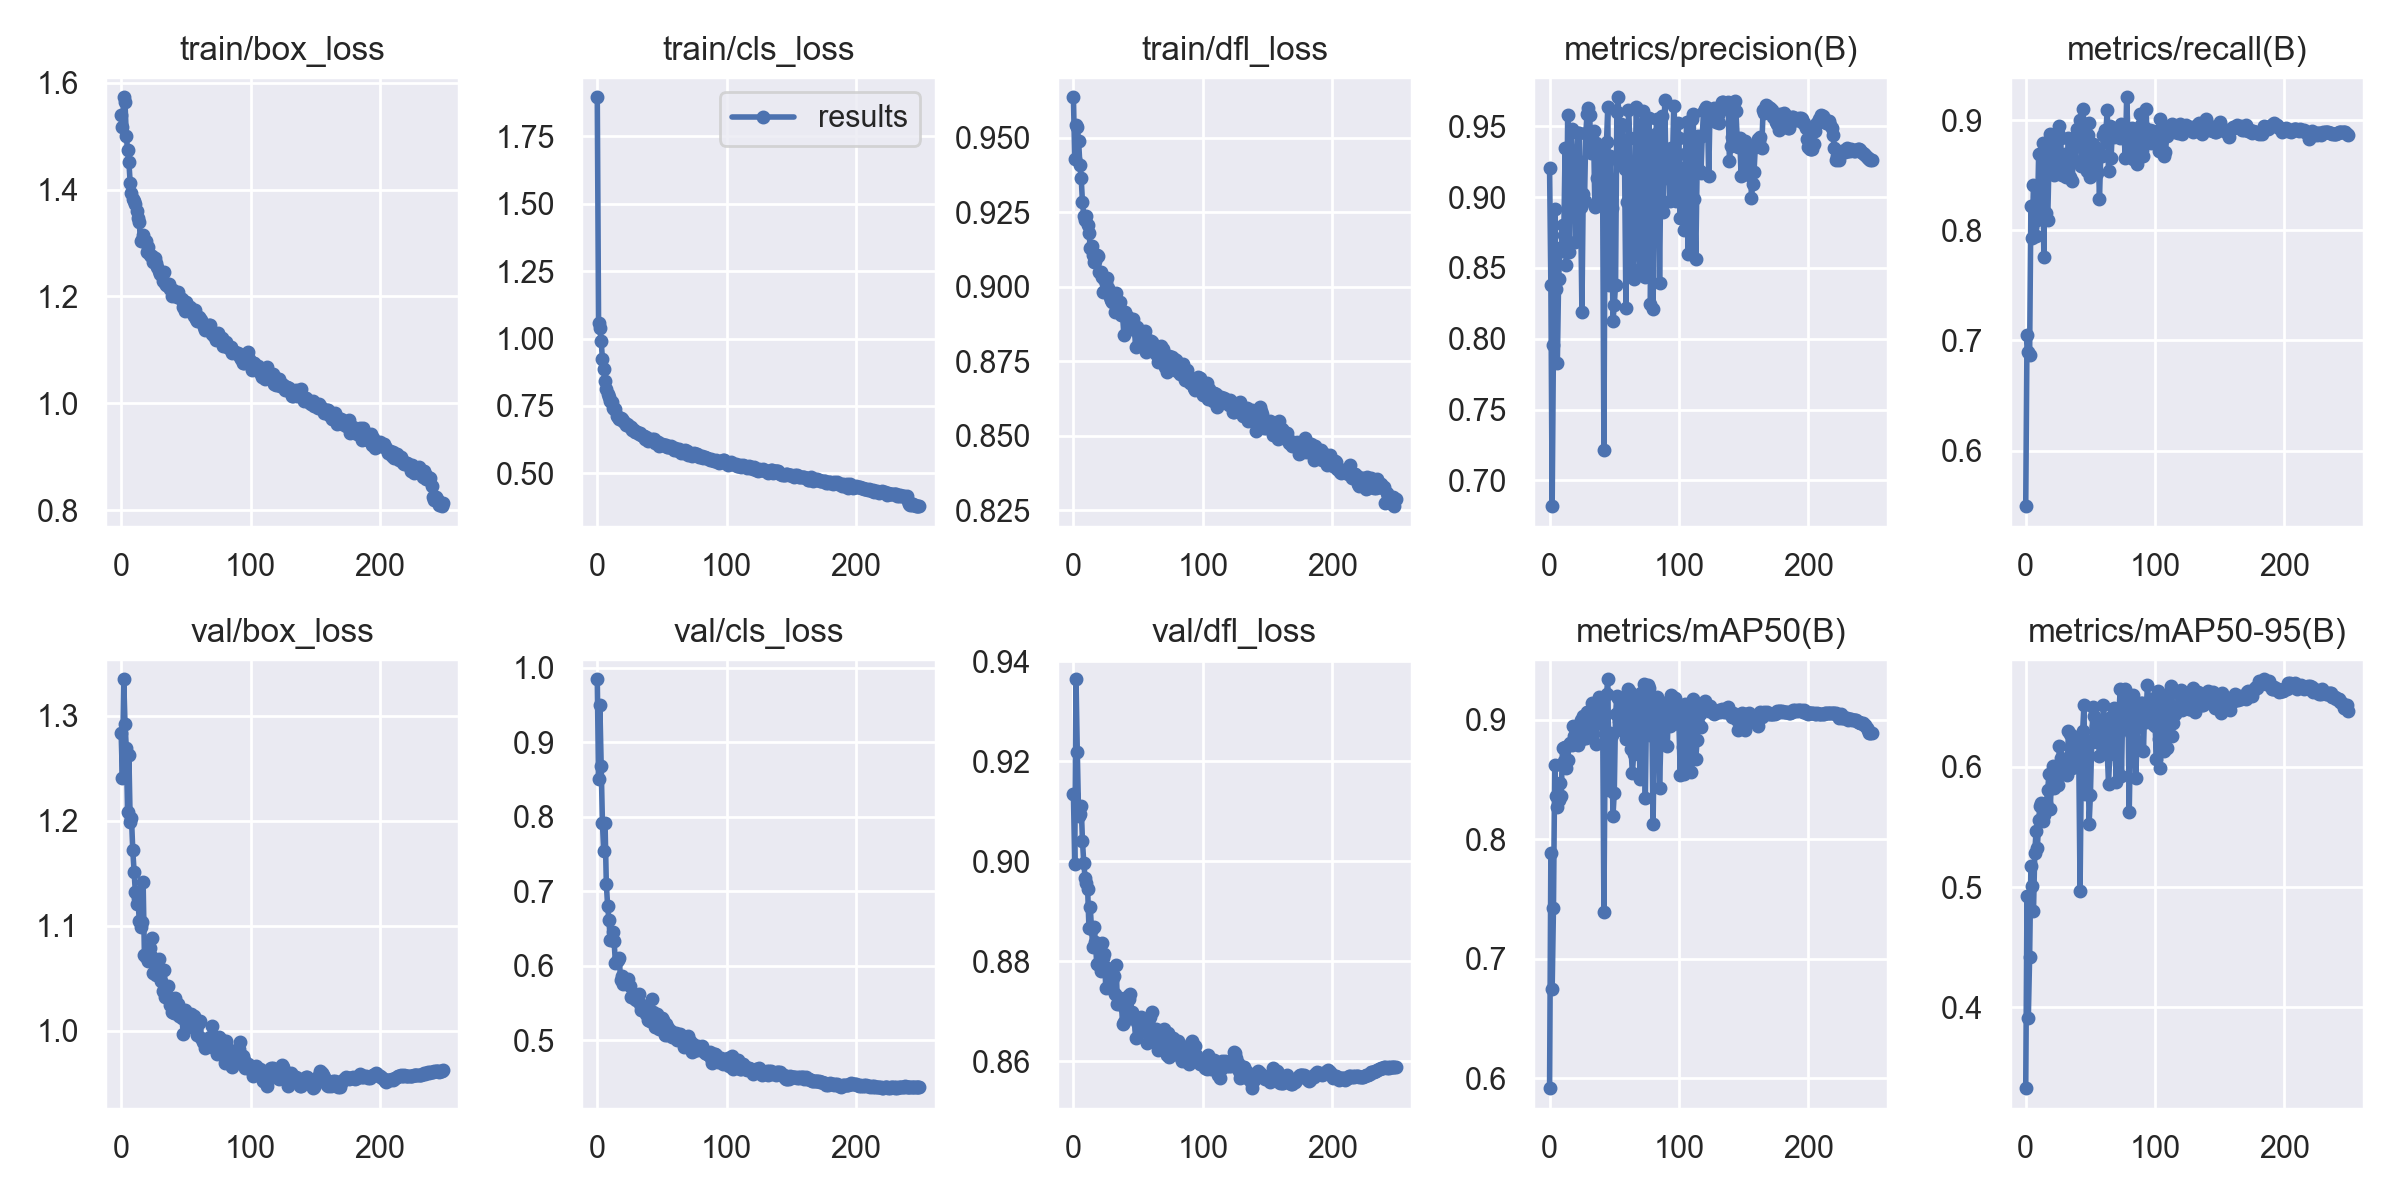
\includegraphics[width=0.45\textwidth]{gambar/grafik_model_malam.png}
\caption{Training curves for the nighttime YOLOv8 model.}
\label{fig:grafik_model_malam}
\end{figure}

Figure~\ref{fig:confusion_matrix_malam} shows the confusion matrix from the nighttime training run.

\begin{figure}[H]
\centering
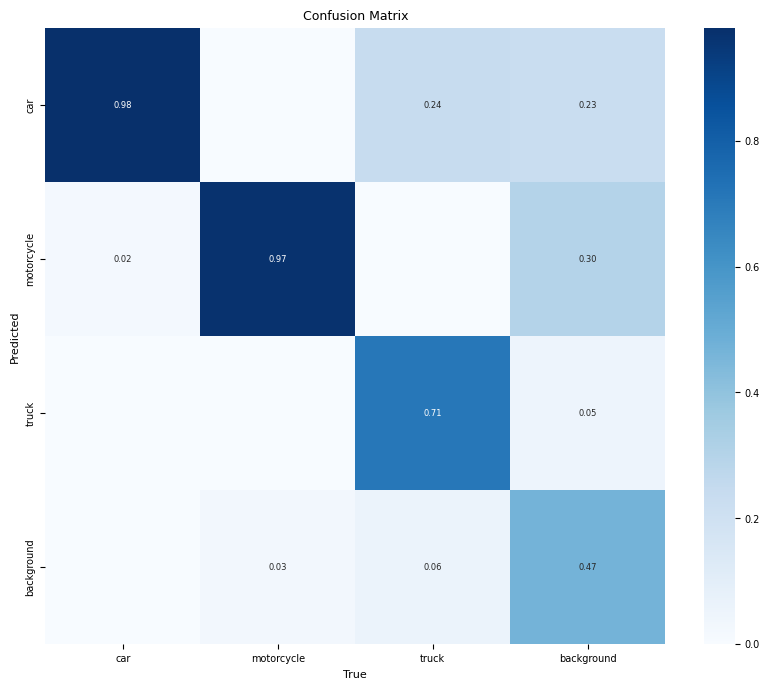
\includegraphics[width=0.45\textwidth]{gambar/confusion_malam.png}
\caption{Confusion matrix of the nighttime detection model.}
\label{fig:confusion_matrix_malam}
\end{figure}

\begin{itemize}
    \item \textbf{Car:} 98\% correct; 2\% misclassified as motorcycle.
    \item \textbf{Motorcycle:} 97\% correct; 3\% predicted as background.
    \item \textbf{Truck:} 71\% correct; 24\% misclassified as car.
    \item \textbf{Background:} Only 47\% correctly identified.
\end{itemize}

Validation results in Figure~\ref{fig:validasi_malam} indicate that smaller objects (motorcycles) yielded lower confidence values (min. 0.5) compared to larger ones (cars, up to 0.9).

\begin{figure}[H]
\centering
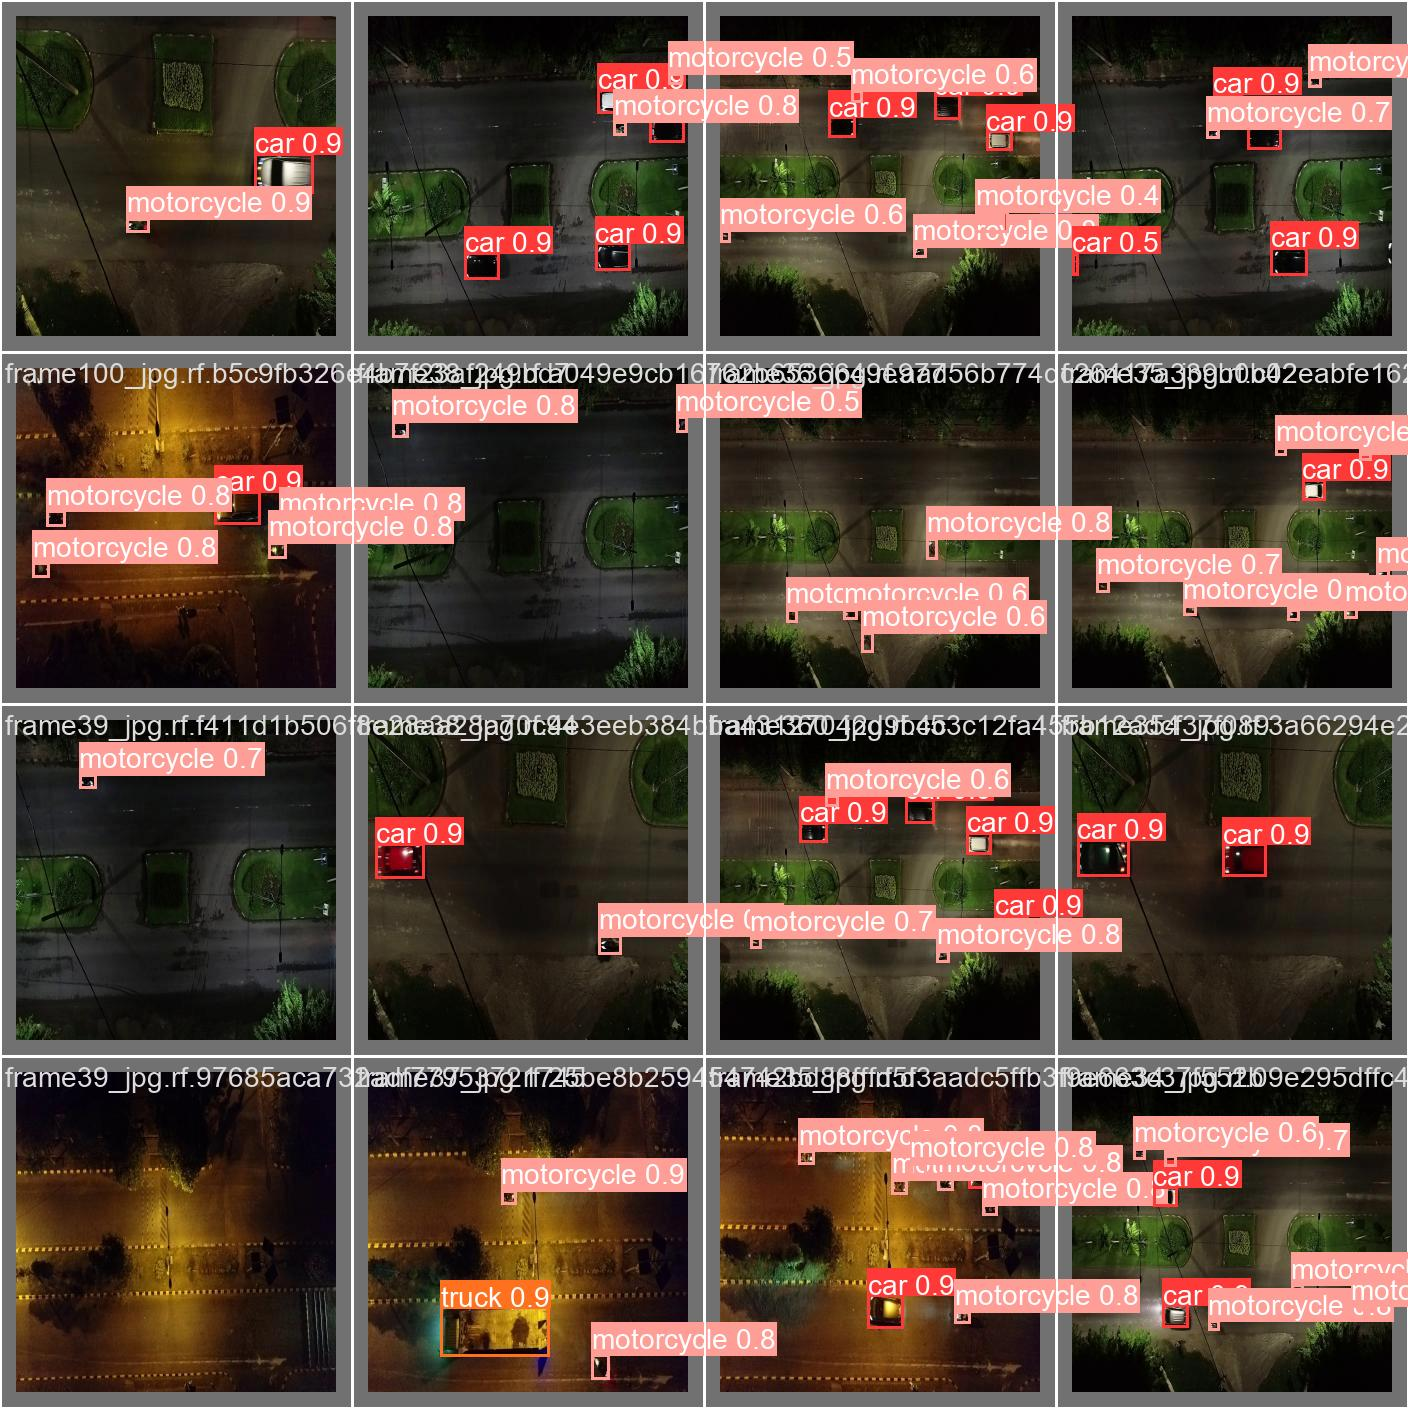
\includegraphics[width=0.45\textwidth]{gambar/val_batch_malam.jpg}
\caption{Validation results for the nighttime model.}
\label{fig:validasi_malam}
\end{figure}

\subsection{Comparison and Evaluation at 20 km/h in Daylight}

This subsection evaluates the system's speed estimation performance at a vehicle speed of 20 km/h in daylight conditions, and compares the results with prior research by Fatchurozi (2024) and Tilon \& Nex (2023).

Experiments were conducted with a motorcycle moving at an average speed of 20 km/h. The drone remained static at altitudes of 20 m, 30 m, and 40 m. Table~\ref{table:manual_speed_calc} shows the manually measured average speed.

\begin{table}[htbp]
\centering
\caption{Manual Speed Calculation at 20 km/h}
\label{table:manual_speed_calc}
\begin{tabular}{|c|c|c|c|c|}
\hline
\textbf{Altitude (m)} & Run 1 & Run 2 & Run 3 & \textbf{Average (km/h)} \\ \hline
20 & 23.33 & 22.90 & 22.30 & 22.84 \\ \hline
30 & 18.94 & 18.80 & 18.76 & 18.83 \\ \hline
40 & 18.81 & 18.79 & 18.72 & 18.77 \\ \hline
\end{tabular}
\end{table}

Table~\ref{table:system_speed_calc} presents the results of the proposed system, including mean and standard deviation.

\begin{table}[htbp]
\centering
\caption{Speed Estimation by Proposed System at 20 km/h}
\label{table:system_speed_calc}
\begin{tabular}{|c|c|c|c|c|c|}
\hline
\textbf{Altitude (m)} & Run 1 & Run 2 & Run 3 & \textbf{Average} & \textbf{Std. Dev.} \\ \hline
20 & 21.59 & 20.06 & 21.61 & 21.09 & 0.72 \\ \hline
30 & 23.28 & 21.25 & 25.05 & 23.19 & 1.55 \\ \hline
40 & 22.24 & 24.39 & 21.70 & 22.78 & 1.16 \\ \hline
\end{tabular}
\end{table}

Error calculations for Trial 1 are shown in Table~\ref{table:error_accuracy_t1}.

\begin{table}[htbp]
\centering
\caption{Error and Accuracy - Trial 1}
\label{table:error_accuracy_t1}
\begin{tabular}{|c|c|c|c|c|}
\hline
\textbf{Altitude (m)} & Error & Absolute Error & Relative Error (\%) & Accuracy (\%) \\ \hline
20 & -1.74 & 1.74 & 7.46 & 92.54 \\ \hline
30 & 4.34 & 4.34 & 22.91 & 77.09 \\ \hline
40 & 3.43 & 3.43 & 18.23 & 81.77 \\ \hline
\end{tabular}
\end{table}

The system showed the highest accuracy at 20 m altitude across all trials. At higher altitudes, reduced pixel density lowered speed estimation accuracy.

Table~\ref{table:accuracy_fatchurozi} summarizes results from Fatchurozi (2024) for 20 km/h scenarios, while Table~\ref{table:accuracy_tilon} shows the accuracy from Tilon \& Nex (2023) at 15 km/h and 50 m altitude.

\begin{table}[htbp]
\centering
\caption{Accuracy Comparison with Fatchurozi (2024)}
\label{table:accuracy_fatchurozi}
\begin{tabular}{|c|c|c|c|}
\hline
\textbf{Altitude (m)} & Trial 1 (\%) & Trial 2 (\%) & Trial 3 (\%) \\ \hline
20 & 89.75 & 90.52 & 88.26 \\ \hline
30 & 93.47 & 91.55 & 87.98 \\ \hline
40 & 86.11 & 94.96 & 89.13 \\ \hline
\end{tabular}
\end{table}

\begin{table}[htbp]
\centering
\caption{Accuracy from Tilon \& Nex (2023) at 15 km/h}
\label{table:accuracy_tilon}
\begin{tabular}{|c|c|}
\hline
\textbf{Altitude (m)} & Accuracy (\%) \\ \hline
50 & 77.59 \\ \hline
\end{tabular}
\end{table}

The proposed system achieved accuracy exceeding 90\% at 20 m altitude, which decreased at higher altitudes. Compared to previous studies, the system performs competitively, particularly at low altitudes. Key influencing factors include altitude, image resolution, and vehicle type. Real-time edge processing on Jetson Nano enhances the system’s applicability in portable deployments.


